\documentclass[a4]{article}
\pagestyle{myheadings}

%%%%%%%%%%%%%%%%%%%
% Packages/Macros %
%%%%%%%%%%%%%%%%%%%
\usepackage{mathrsfs}


\usepackage{fancyhdr}
\pagestyle{fancy}
\lhead{}
\chead{}
\rhead{}
\lfoot{}
\cfoot{} 
\rfoot{\normalsize\thepage}
\renewcommand{\headrulewidth}{0pt}
\renewcommand{\footrulewidth}{0pt}
\newcommand{\RomanNumeralCaps}[1]
{\MakeUppercase{\romannumeral #1}}

\usepackage{amssymb,latexsym}  % Standard packages
\usepackage[utf8]{inputenc}
\usepackage[russian]{babel}
\usepackage{MnSymbol}
\usepackage{amsmath,amsthm}
\usepackage{indentfirst}
\usepackage{graphicx}%,vmargin}
\usepackage{graphicx}
\graphicspath{{pictures/}} 
\usepackage{verbatim}
\usepackage{color}









\DeclareGraphicsExtensions{.pdf,.png,.jpg}% -- настройка картинок

\usepackage{epigraph} %%% to make inspirational quotes.
\usepackage[all]{xy} %for XyPic'a
\usepackage{color} 
\usepackage{amscd} %для коммутативных диграмм


\newtheorem{Lemma}{Лемма}[section]
\newtheorem{Proposition}{Предложение}[section]
\newtheorem{Theorem}{Теорема}[section]
\newtheorem{Corollary}{Следствие}[section]
\newtheorem{Remark}{Замечание}[section]
\newtheorem{Definition}{Определение}[section]
\newtheorem{Designations}{Обозначение}[section]




%%%%%%%%%%%%%%%%%%%%%%%% 
%Сношение с оглавлением% 
%%%%%%%%%%%%%%%%%%%%%%%% 
\usepackage{tocloft} 
\renewcommand{\cftdotsep}{2} %частота точек
\renewcommand\cftsecleader{\cftdotfill{\cftdotsep}}
\renewcommand{\cfttoctitlefont}{\hspace{0.38\textwidth} \LARGE\bfseries} 
\renewcommand{\cftsecaftersnum}{.}
\renewcommand{\cftsubsecaftersnum}{.}
\renewcommand{\cftbeforetoctitleskip}{-1em} 
\renewcommand{\cftaftertoctitle}{\mbox{}\hfill \\ \mbox{}\hfill{\footnotesize Стр.}\vspace{-0.5em}} 
\renewcommand{\cftsubsecfont}{\hspace{1pt}} 
\renewcommand{\cftparskip}{3mm} %определяет величину отступа в оглавлении
\setcounter{tocdepth}{5} 




\addtolength{\textwidth}{0.7in}
\textheight=630pt
\addtolength{\evensidemargin}{-0.4in}
\addtolength{\oddsidemargin}{-0.4in}
\addtolength{\topmargin}{-0.4in}

\newcommand{\empline}{\mbox{}\newline} 
\newcommand{\likechapterheading}[1]{ 
	\begin{center} 
		\textbf{\MakeUppercase{#1}} 
	\end{center} 
	\empline} 

\makeatletter 
\renewcommand{\@dotsep}{2} 
\newcommand{\l@likechapter}[2]{{\bfseries\@dottedtocline{0}{0pt}{0pt}{#1}{#2}}} 
\makeatother 
\newcommand{\likechapter}[1]{ 
	\likechapterheading{#1} 
	\addcontentsline{toc}{likechapter}{\MakeUppercase{#1}}} 





\usepackage{xcolor}
\usepackage{hyperref}
\definecolor{linkcolor}{HTML}{000000} % цвет ссылок
\definecolor{urlcolor}{HTML}{AA1622} % цвет гиперссылок

\hypersetup{pdfstartview=FitH,  linkcolor=linkcolor,urlcolor=urlcolor, colorlinks=true}



\def \newstr {\medskip \par \noindent} 



\begin{document}
	\def\contentsname{\LARGE{Содержание}}
	\thispagestyle{empty}
	\begin{center} 
		\vspace{2cm} 
		{\Large \sc Санкт-Петербургский Политехнический Университет}\\
		\vspace{2mm}
		{\Large\sc Петра Великого}\\
		\vspace{1cm}
		{\large \sc Институт прикладной математики и механики\\ 
			\vspace{0.5mm}
			\textsc{}}\\ 
		\vspace{0.5mm}
		{\large\sc Кафедра $"$Прикладная математика$"$}\\
		\vspace{15mm}
		
		
		{\sc \textbf{Отчёт\\
			Лабораторная работа №$5$\\
			по дисциплине\\
			"Математическая статистика"}
			\vspace{6mm}
			
		}
		\vspace*{2mm}
		
		
		\begin{flushleft}
			\vspace{4cm}
			\sc Выполнил студент:\\
			\sc Салихов С.Р.\\
			\sc группа: 3630102/70401\\
			\vspace{1cm}
			\sc Проверил:\\
			\sc к.ф-м.н., доцент\\
			\sc Баженов Александр Николавич
			\vspace{20mm}
		\end{flushleft}
	\end{center} 
	\begin{center}
		\vfill {\large\textsc{Санкт-Петербург}}\\ 
		2020 г.
	\end{center}
	
	\newpage
	\pagestyle{plain}
	
	%\begin{center}
	%\begin{abstract} 
	
	%\end{abstract}
	
	%\end{center}
	
	\newpage
	\tableofcontents{}
	\newpage
	\listoffigures
	\newpage
	\listoftables
	\newpage
	
	
	\section{Постановка задачи}
		Сгенерировать двумерные выборки размерами 20, 60, 100 для нормального двумерного распределения N(x, y, 0, 0, 1, 1, $\rho$).\\
		Коэффициент корреляции $\rho$ взять равным 0, 0.5, 0.9.\\
		Каждая выборка генерируется 1000 раз и для неё вычисляются: среднее значение, среднее значение квадрата и дисперсия коэффициентов корреляции Пирсона, Спирмена и квадрантного коэффициента корреляции.
		Повторить все вычисления для смеси нормальных распределений:

		$$f(x, y) = 0.9N(x, y, 0, 0, 1, 1, 0.9) + 0.1N(x, y, 0, 0, 10, 10, -0.9).$$
		Изобразить сгенерированные точки на плоскости и нарисовать эллипс равновероятности.
	\section{Теория}
		\subsection{Двумерное нормальное распределение}
			Двумерная случайная величина (X, Y) называется распределённой нормально (или просто нормальной), если её плотность вероятности определена
			формулой
			
			$$N(x, y, \overline{x}, \overline{y}, \delta_x, \delta_y, \rho) = \frac{1}{2\pi\delta_x\delta_y\sqrt{1 - \rho^2}} * exp\left\{
			\begin{array}{ccc}
			-\frac{1}{2(1 - \rho^2)} [\frac{(x - \overline{x})^2}{\delta^2_x} - 2\rho\frac{(x - \overline{x})(y - \overline{y})}{\delta_x \delta_y} + \frac{(y - \overline{y})^2}{\delta^2_y}]
			\end{array}
			\right\}$$
			
			Компоненты X, Y двумерной нормальной случайной величины также распределены нормально с математическими ожиданиями x, y и средними квадратическими отклонениями $\delta_x$, $\delta_y$ соответственно. \\
			Параметр $\rho$ называется коэффициентом корреляции.
		
		\subsection{Корреляционный момент(ковариация) и коэффициент корреляции}
			Корреляционным моментом, иначе ковариацией, двух случайных величин X и Y называется математическое ожидание произведения отклонений этих случайных величин от их математических ожиданий.
			
			$$K = cov(X, Y) = M[(X - \overline{x})(Y - \overline{y})]$$
			
			Коэффициентом корреляции $\rho$ двух случайных величин X и Y называется отношение их корреляционного момента к произведению их средних квадратических отклонений:
			$$\rho = \frac{K}{\delta_x\delta_y}$$

			
			Коэффициент корреляции — это нормированная числовая характеристика, являющаяся мерой близости зависимости между случайными величинами
			к линейной.
			
			\subsection{Выборочные коэффициенты корреляции}
				\subsubsection{Выборочный коэффициент корреляции Пирсона}
					
Пусть по выборке значений 
					

					
$\{{x_i, y_i}\}^n_1$ 1 двумерной с.в. (X, Y ) требуется оценить коэффициент корреляции $\rho$ = $\frac{cov(X, Y)}{\sqrt{DX DY}}$. Естественной оценкой для $\rho$ служит его статистический аналог в виде выборочного коэффициента корреляции, предложенного К.Пирсоном, —
					

					
$$r = \frac{\frac{1}{n} \sum(x_i - \overline{x})(y_i - \overline{y})}{\sqrt{\frac{1}{n} \sum (x_i - \overline{x})^2 \frac{1}{n} \sum(y_i - \overline{y})^2})} = \frac{K}{s_X s_Y}$$
					
где K, $s^2_X, s^2_Y$ - выборочные ковариации и дисперсии с.в. X и Y.
					

					
\subsubsection{Выборочный квадрантный коэффициент корреляции}
					
	Кроме выборочного коэффициента корреляции Пирсона, существуют и другие оценки степени взаимосвязи между случайными величинами. К ним относится выборочный квадрантный коэффициент корреляции
					
	$$r_Q = \frac{(n_1 + n_3) - (n_2 + n_4)}{n}$$
					
	
					
	где $n_1, n_2, n_3 и n_4$ - количества точке с координатами $(x_i, y_i)$, попавшими
					
	соответственно в I, II, III и IV квадранты декартовой системы с осями $x' = x - med x, y' = y - med y$ и с центром в точке с координатами (med x, med y).
					
					\subsubsection{Выборочный коэффициент ранговой корреляции Спирмена}
						На практике нередко требуется оценить степень взаимодействия между качественными признаками изучаемого объекта. Качественным называется признак, который нельзя измерить точно, но который позволяет сравнивать изучаемые объекты между собой и располагать их в порядке убывания или возрастания их качества. Для этого объекты выстраиваются в определённом порядке в соответствии с рассматриваемым признаком. Процесс упорядочения называется ранжированием, и каждому члену упорядоченной последовательности объектов присваивается ранг, или порядковый номер. Например, объекту с наименьшим значением признака присваивается ранг 1, следующему за ним объекту — ранг 2, и т.д. Таким образом, происходит сравнение каждого объекта со всеми объектами изучаемой выборки.\\
						
						Если объект обладает не одним, а двумя качественными признаками — переменными X и Y , то для исследования их взаимосвязи используют выборочный коэффициент корреляции между двумя последовательностями рангов этих признаков.\\
						Обозначим ранги, соотвествующие значениям переменной X, через u, а ранги, соотвествующие значениям переменной Y , — через $\upsilon$.\\
						Выборочный коэффициент ранговой корреляции Спирмена определяется как выборочный коэффициент корреляции Пирсона между рангами u, $\upsilon$ переменных X, Y :
						
						$$r = \frac{\frac{1}{n} \sum(u_i - \overline{u})(\upsilon_i - \overline{\upsilon})}{\sqrt{\frac{1}{n} \sum (u_i - \overline{u})^2 \frac{1}{n} \sum(\upsilon_i - \overline{\upsilon})^2})}$$
						где $\overline{u} = \overline{\upsilon} = \frac{1 + 2 + .. + n}{n} = \frac{n + 1}{2}$ - среднее значение рангов.
	\section{Реализация}
	Для генерации выборки был использован $Python\;3.7$ и модуль numpy. Для отрисовки графиков использовался модуль matplotlib. scipy.stats для обработки функций распределений.
	\section{Результаты}
		\subsection{Выборочные коэффициенты корреляции}
		\begin{table}[h!]
			
			\caption{Результаты для двумерного нормального распределения при  n = 20}
			\label{tab:my_label}
			\begin{center}
				\vspace{5mm}
				\begin{tabular}{|c|c|c|c}
					\hline
					$\rho$ = 0 & r & $r_S$ & $r_Q$ \\
					\hline
					E(z) & -0.005 & -0.004 & -0.002\\
					\hline
					E($z^2$)   & 0.057 & 0.057 & 0.056\\
					\hline
					D(z)   & 0.057 & 0.057 & 0.056 \\
					\hline
					$\rho$ = 0.5 & r & $r_S$ & $r_Q$ \\
					\hline\\
					\hline
					E(z) & 0.481 & 0.455 & 0.315\\
					\hline
					E($z^2$)   & 0.263 & 0.242 & 0.148\\
					\hline
					D(z)   & 0.031 & 0.034 & 0.048 \\
					\hline
					$\rho$ = 0.9 & r & $r_S$ & $r_Q$ \\
					\hline\\
					\hline
					E(z) & 0.897 & 0.866 & 0.699\\
					\hline
					E($z^2$)   & 0.808 & 0.754 & 0.516\\
					\hline
					D(z)   & 0.002 & 0.004 & 0.027 \\
					\hline
				\end{tabular}
				
			\end{center}
			
		\end{table}
		
		\begin{table}[h!]
			
			\caption{Результаты для двумерного нормального распределения при  n = 60}
			\label{tab:my_label}
			\begin{center}
				\vspace{5mm}
				\begin{tabular}{|c|c|c|c}
					\hline
					$\rho$ = 0 & r & $r_S$ & $r_Q$ \\
					\hline
					E(z) & -0.002 & -0.002 & -0.001\\
					\hline
					E($z^2$)   & 0.016 & 0.017 & 0.017\\
					\hline
					D(z)   & 0.016 & 0.017 & 0.017 \\
					\hline
					$\rho$ = 0.5 & r & $r_S$ & $r_Q$ \\
					\hline\\
					\hline
					E(z) & 0.499 & 0.477 & 0.328\\
					\hline
					E($z^2$)   & 0.258 & 0.238 & 0.122\\
					\hline
					D(z)   & 0.009 & 0.010 & 0.014 \\
					\hline
					$\rho$ = 0.9 & r & $r_S$ & $r_Q$ \\
					\hline\\
					\hline
					E(z) & 0.898 & 0.881 & 0.704\\
					\hline
					E($z^2$)   & 0.807 & 0.779 & 0.504\\
					\hline
					D(z)   & 0.0007 & 0.0011 & 0.008 \\
					\hline
				\end{tabular}
				
			\end{center}
			
		\end{table}
		\newpage
		\begin{table}[h!]
			
			\caption{Результаты для двумерного нормального распределения при  n = 100}
			\label{tab:my_label}
			\begin{center}
				\vspace{5mm}
				\begin{tabular}{|c|c|c|c}
					\hline
					$\rho$ = 0 & r & $r_S$ & $r_Q$ \\
					\hline
					E(z) & -0.004 & -0.004 & -0.002\\
					\hline
					E($z^2$)   & 0.009 & 0.009 & 0.1\\
					\hline
					D(z)   & 0.009 & 0.009 & 0.010 \\
					\hline
					$\rho$ = 0.5 & r & $r_S$ & $r_Q$ \\
					\hline\\
					\hline
					E(z) & 0.496 & 0.477 & 0.330\\
					\hline
					E($z^2$)   & 0.252 & 0.234 & 0.117\\
					\hline
					D(z)   & 0.006 & 0.006 & 0.009 \\
					\hline
					$\rho$ = 0.9 & r & $r_S$ & $r_Q$ \\
					\hline\\
					\hline
					E(z) & 0.899 & 0.887 & 0.710\\
					\hline
					E($z^2$)   & 0.809 & 0.787 & 0.510\\
					\hline
					D(z)   & 0.0004 & 0.0006 & 0.005 \\
					\hline
				\end{tabular}
				
			\end{center}
			
		\end{table}
		
		\begin{table}[h!]
			
			\caption{Смесь нормальных распределений}
			\label{tab:my_label}
			\begin{center}
				\vspace{5mm}
				\begin{tabular}{|c|c|c|c}
					\hline
					n = 20 & r & $r_S$ & $r_Q$ \\
					\hline
					E(z) & 0.384 & 0.364 & 0.251\\
					\hline
					E($z^2$)   & 0.187 & 0.174 & 0.113\\
					\hline
					D(z)   & 0.039 & 0.042 & 0.051 \\
					\hline
					n = 60 & r & $r_S$ & $r_Q$ \\
					\hline\\
					\hline
					E(z) & 0.397 & 0.378 & 0.260\\
					\hline
					E($z^2$)   & 0.170 & 0.156 & 0.084\\
					\hline
					D(z)   & 0.012 & 0.013 & 0.016 \\
					\hline
					n = 100 & r & $r_S$ & $r_Q$ \\
					\hline\\
					\hline
					E(z) & 0.397 & 0.380 & 0.259\\
					\hline
					E($z^2$)   & 0.165 & 0.152 & 0.077\\
					\hline
					D(z)   & 0.007 & 0.008 & 0.009 \\
					\hline
				\end{tabular}
				
			\end{center}
			
		\end{table}
	\newpage
	\subsection{Эллипсы рассеивания}
		\begin{center}
			
			\begin{figure}[h!]
				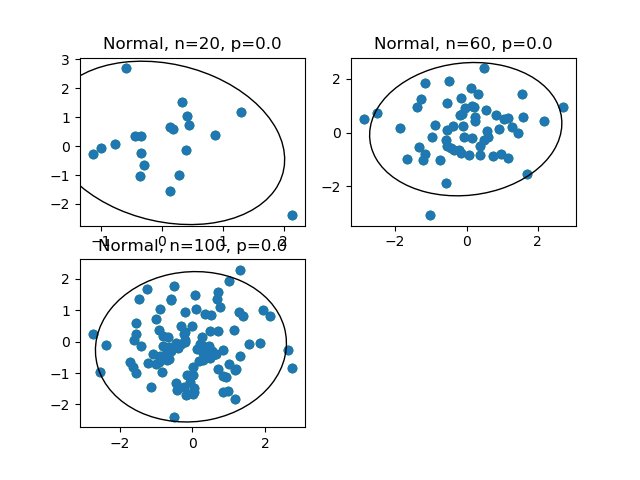
\includegraphics[width=\textwidth]{Normal0.png} 
				\caption[Двумерное нормальное распределение, при $\rho$ = 0]{Двумерное нормальное распределение, при $\rho$ = 0}
			\end{figure}
			\newpage
			\begin{figure}[h!]
				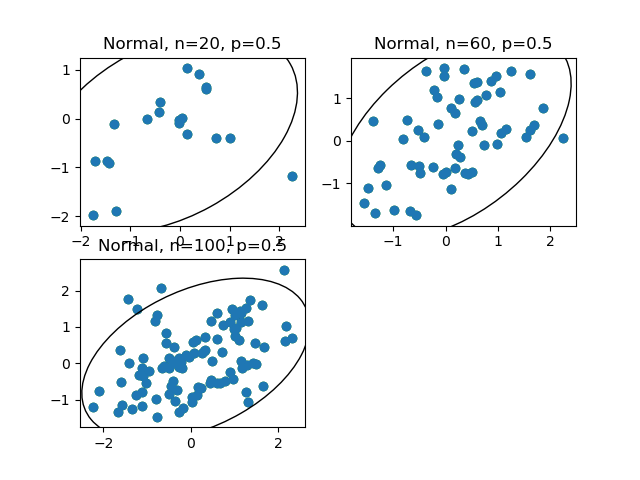
\includegraphics[width=\textwidth]{Normal5.png} 
				\caption[Двумерное нормальное распределение, при $\rho$ = 0.5]{Двумерное нормальное распределение, при $\rho$ = 0.5}
			\end{figure}
			\newpage
			\begin{figure}[h!]
				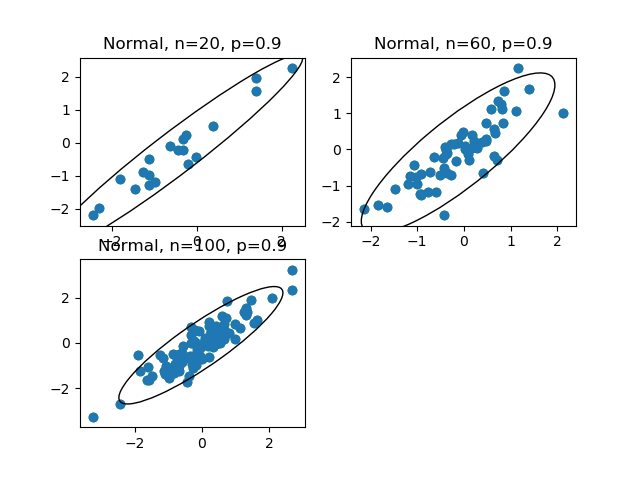
\includegraphics[width=\textwidth]{Normal9.png} 
				\caption[Двумерное нормальное распределение, при $\rho$ = 0.9]{Двумерное нормальное распределение, при $\rho$ = 0.9}
			\end{figure}
			\newpage
			\begin{figure}[h!]
				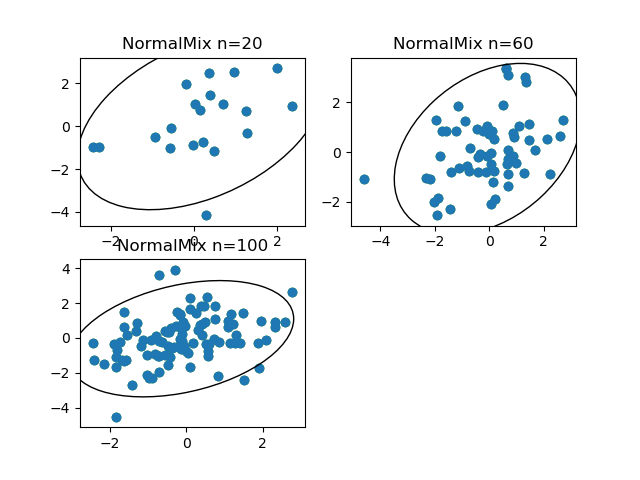
\includegraphics[width=\textwidth]{NormalMix9.png} 
				\caption[Смесь нормальных распределений]{Смесь нормальных распределений}
			\end{figure}
			
		\end{center}
			
	\section{Обсуждение}
		\subsection{Выборочные коэффициенты корреляции и эллипсы рассеивания}
			1)Сравним дисперсии выборочных коэффициентов корреляции.\\
			– Для двумерного нормального распределения дисперсии выборочных коэффициентов корреляции упорядочены следующим образом: r < $r_S$ < $r_Q$.\\
			– Для смеси нормальных распределений дисперсии выборочных
			коэффициентов корреляции упорядочены следующим образом:
			$r_Q$ < $r_S$ < r.\\
			
			2)Процент попавших элементов выборки в эллипс рассеивания ($95%$-я доверительная область) примерно равен его теоретическому значению
			($95%$).
		\subsection{Стравнение с теоретическими данными}
		По таблицам видно, что при увеличении объёма выборки, подсчитанные коэффициенты стремятся к теоретическим.\\
		По графикам видно, что при уменьшении корреляции эллипс равновероятности стремится к окружности, а при увеличении растягивается.
	\section{Литература}
	
	\href{https://physics.susu.ru/vorontsov/language/numpy.html}{Модуль numpy}\\
	
	\href{https://matplotlib.org/}{Модуль matplotlib}\\
	
	\href{https://www.scipy.org/}{Модуль scipy}\\
	
	
	\href{https://ru.wikipedia.org/wiki/%D0%9C%D0%BD%D0%BE%D0%B3%D0%BE%D0%BC%D0%B5%D1%80%D0%BD%D0%BE%D0%B5_%D0%BD%D0%BE%D1%80%D0%BC%D0%B0%D0%BB%D1%8C%D0%BD%D0%BE%D0%B5_%D1%80%D0%B0%D1%81%D0%BF%D1%80%D0%B5%D0%B4%D0%B5%D0%BB%D0%B5%D0%BD%D0%B8%D0%B5}{Многомерное нормальное распределение}
	
	\href{https://ru.wikipedia.org/wiki/%D0%9A%D0%BE%D1%80%D1%80%D0%B5%D0%BB%D1%8F%D1%86%D0%B8%D1%8F}{Корреляция}
	
	
	\section{Приложения}
	
	\href{https://github.com/LuciusGen/Matstat/blob/master/Lab5/Lab5.py}{Код лаборатрной}
	
	\href{https://github.com/LuciusGen/Matstat/blob/master/Lab5/lab5.tex}{Код отчёта}
	
\end{document}